\documentclass[conference]{IEEEtran}
\usepackage{cite}
\usepackage{amsmath,amssymb,amsfonts}
\usepackage{algorithmic}
\usepackage{graphicx}
\usepackage{textcomp}
\usepackage{xcolor}
\usepackage{booktabs}
\usepackage{tabularx}
\usepackage{url}
\usepackage{hyperref}

\hypersetup{
    hidelinks,
    colorlinks=false,
    pdfborder={0 0 0}
}

\begin{document}
\setlength{\textfloatsep}{6pt plus 1pt minus 1pt}
\setlength{\floatsep}{6pt plus 1pt minus 1pt}
\setlength{\intextsep}{6pt plus 1pt minus 1pt}


\title{recovery\_eval: State-Matched and Provenance-Aware Evaluation of Recovery Behavior in Language-Model Reasoning}

\author{\IEEEauthorblockN{Sham Satish Thakare}
\IEEEauthorblockA{\textit{Independent Researcher} \\
Pune, Maharashtra, India \\
Email: shamthakare@gmail.com}
}

\maketitle

\begin{abstract}
Evaluating whether instruction-tuned language models exhibit genuine error-recovery capabilities in multi-step reasoning is challenging because improvements in overall continuation fluency confound recovery-specific adaptation. We introduce \texttt{recovery\_eval}, a data-centric evaluation methodology designed to evaluate model recovery-state continuation behavior relative to reference controls via an interaction contrast ($D_{\text{recovery}}$). The framework integrates paired counterfactual prefix perturbation with an immutable append-only exposure ledger, full token generation provenance, and deterministic symbolic verifier execution. We evaluate \texttt{recovery\_eval} across 400 neural continuations generated by two released \texttt{Qwen2.5-Math-1.5B} checkpoint-interface configurations (Base with plain-text completion and Instruct with ChatML formatting) across 20 prospectively generated arithmetic reasoning problems using five prespecified random seeds under stochastic sampling ($T=0.7$, $p=0.9$, 64-token cap). Output diversity audits confirm 98.75\% unique continuations per 5-seed cell (4.99/5.0 mean). On recovery states, continuation success improved from 0.2100 (Base) to 0.6400 (Instruct) ($+0.4300$), while on matched control states, success improved from 0.3800 to 0.9200 ($+0.5400$). The resulting additive interaction contrast was $D_{\text{recovery}} = -0.1100$, with a 95\% problem-cluster bootstrap confidence interval of $[-0.240, +0.030]$ (10,000 resamples, $p \approx 0.122$; cluster paired $t$-test $p=0.1419$; permutation $p=0.1759$). Instruction tuning demonstrated no statistically detectable recovery-specific advantage over Base beyond baseline fluency gains. Furthermore, diagnostic sensitivity analysis reveals that $D_{\text{recovery}}$ is heavily dictated by verifier regex assumptions (shifting from $-0.2000$ to $-0.0200$ across extraction rules) and generation horizon truncation (53.0\% overall; 83.0\% on Base Recovery). A stratified $N=100$ verifier validation study reveals 100\% precision but a 42.1\% false negative penalty on Base models. We conclude with practical methodological recommendations and pre-register a prospective 256-token balanced protocol for future benchmark design.
\end{abstract}

\begin{IEEEkeywords}
Large Language Models, Mathematical Reasoning, Error Recovery, Model Evaluation, Data-Centric AI, Reproducibility
\end{IEEEkeywords}

\section{Introduction}
Large language models (LLMs) post-trained on mathematical reasoning achieve high accuracy on standard benchmarks \cite{cobbe2021gsm8k, qwen25math2024}. However, an open research question is whether post-training confers specialized mechanisms for recovering from intermediate logical and arithmetic errors, or whether observed performance gains merely reflect uniform improvements in baseline generation fluency \cite{lightman2023process, zelikman2022star, madaan2023selfrefine, huang2023large, kumar2024training}.

Evaluating error recovery is methodologically challenging. Standard benchmarks measure end-to-end task completion from unperturbed prompts. When models are evaluated on prefixes containing reasoning errors, raw accuracy conflates baseline completion capability with recovery resilience. For instance, an instruction-tuned model may solve more problems following an erroneous prefix simply because its baseline generation quality is universally higher across all prompt contexts, even if its relative sensitivity to reasoning corruption is unchanged or worse.

To address this evaluative challenge, we present \texttt{recovery\_eval}, an open, reproducible framework designed to evaluate model continuation behavior following reasoning perturbations. Our primary contributions are:
\begin{enumerate}
    \item \textbf{Paired Contrast Estimand ($D_{\text{recovery}}$)}: A formal double-difference interaction estimand comparing continuation success across perturbed and control prefix states.
    \item \textbf{Reasoning Outcome Taxonomy}: An operational measurement framework separating terminal accuracy ($Y_{\text{acc}}$) into observable recovery categories (R1--R6): explicit detection, explicit correction, silent recalculation, unverifiable success, failure, and truncation.
    \item \textbf{Evidence Governance Architecture}: An append-only exposure ledger recording token-level generation provenance, model weight manifests, and deterministic symbolic verifier checks.
    \item \textbf{Empirical Diagnostic Findings}: A 400-continuation empirical study on \texttt{Qwen2.5-Math-1.5B} Base and Instruct checkpoints, demonstrating that large observed gains on recovery prefixes ($+0.4300$) were outpaced by gains on matched controls ($+0.5400$), resulting in $D_{\text{recovery}} = -0.1100$ (95\% CI $[-0.240, +0.030]$).
    \item \textbf{Truncation \& Verifier Sensitivity Diagnostics}: Forensic identification of verifier extraction fallbacks and horizon truncation as major confounders, supported by a stratified $N=100$ verifier validation audit.
\end{enumerate}

\begin{figure}[htbp]
\centering
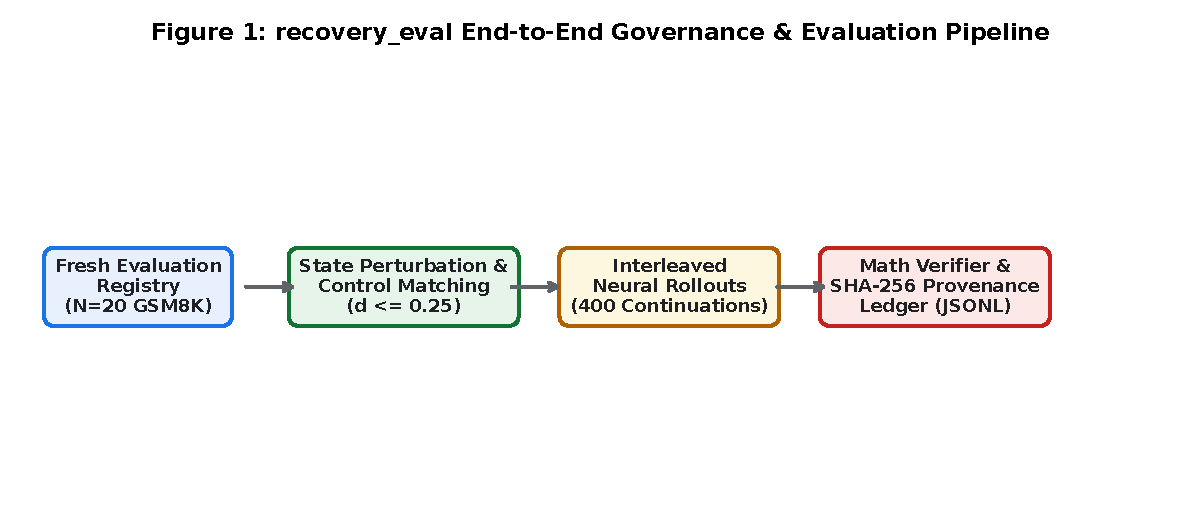
\includegraphics[width=0.86\columnwidth]{figures/fig1_architecture.pdf}
\caption{\texttt{recovery\_eval} End-to-End Governance and Evaluation Pipeline.}
\label{fig:architecture}
\end{figure}

\section{Related Work}

\subsection{Error Detection vs. Self-Correction}
Recent research investigates whether LLMs can identify and rectify their own errors. Tyen et al. \cite{tyen2024llms} introduced BIG-Bench Mistake, showing that while models struggle to locate reasoning errors autonomously, their ability to correct mistakes improves significantly when provided with external error locations. Similarly, Huang et al. \cite{huang2023large} demonstrated that intrinsic multi-turn self-correction without external feedback often degrades accuracy due to spurious self-doubt. Unlike multi-turn prompting benchmarks, \texttt{recovery\_eval} evaluates single-turn generative continuation directly from mid-derivation corrupted prefix states without explicit error warnings.

\subsection{Process Supervision and Benchmark Perturbations}
Process-supervised reward models (PRMs) evaluate reasoning step-by-step \cite{lightman2023process, wang2024mathshepherd}. Zheng et al. \cite{zheng2024processbench} introduced ProcessBench to benchmark the ability of PRMs to identify the earliest erroneous step in mathematical problem solving. While ProcessBench evaluates passive error \textit{identification}, \texttt{recovery\_eval} evaluates generative \textit{continuation success} once placed into an erroneous state. Our approach also relates to input perturbation methods in natural language processing \cite{ribeiro2020beyond, gardner2020evaluating}, extending them to multi-step reasoning prefixes with structural covariate balance.

\subsection{Evaluative Confounding and Baseline Conditioning}
Evaluating models on perturbed inputs without conditioning on baseline shifts is a known source of evaluative confounding \cite{madaan2023selfrefine, shinn2023reflexion}. By formulating a difference-in-differences interaction against matched reference controls, \texttt{recovery\_eval} explicitly controls for general generation capability.

\section{Methodology and Problem Formulation}

\subsection{State Definitions and Perturbation Model}
Let $x$ denote a mathematical problem with ground truth $y^*$. A reasoning trajectory consists of discrete steps $\tau = (s_1, \dots, s_T)$.
\begin{itemize}
    \item \textbf{Reference Control State ($s_C$)}: A valid prefix $s_{1:k}^C$ where all steps up to index $k$ are mathematically sound. In our pilot benchmark pairs, reference control prefixes present completed derivations serving as baseline controls for answer formatting and echoing.
    \item \textbf{Recovery State ($s_R$)}: An identical prefix up to step $k-1$, where step $k$ introduces a controlled local arithmetic perturbation (e.g., $a \times b = c \rightarrow a \times b = c'$ with $c' \ne c$), requiring the model to recalculate the answer.
\end{itemize}
Although the evaluation matches selected prefix characteristics, the control and recovery conditions differ in answer availability. In the evaluated protocol, control prefixes presented completed derivations containing the ground-truth value, whereas recovery prefixes contained injected arithmetic errors without answer exposure. Consequently, the interaction contrast is a descriptive comparison under the constructed protocol, not an identified causal effect of reasoning recovery.

\begin{figure}[htbp]
\centering
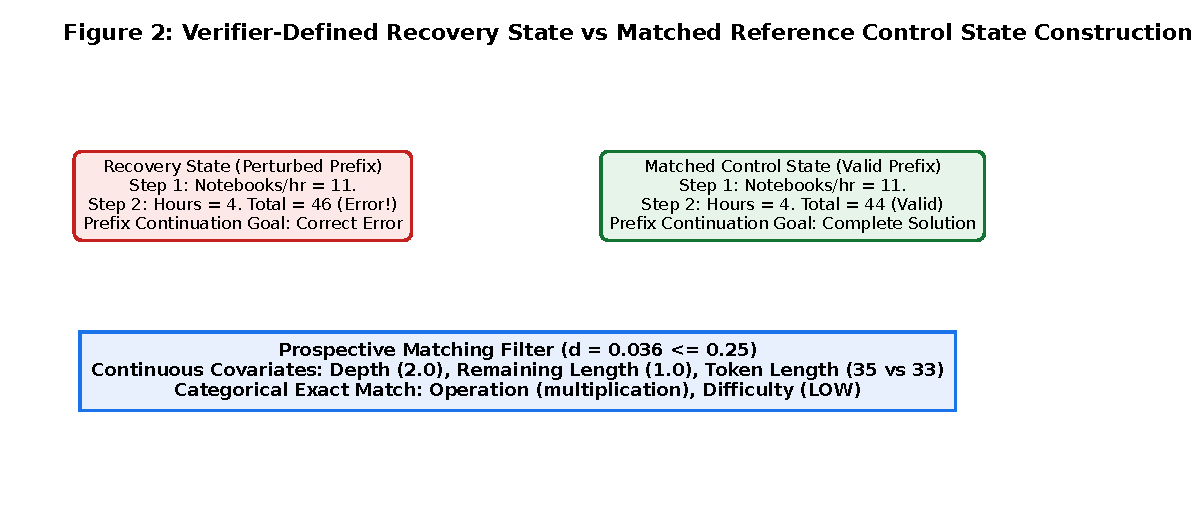
\includegraphics[width=0.85\columnwidth]{figures/fig2_state_construction.pdf}
\caption{Verifier-Defined Recovery State vs. Matched Reference Control State Construction.}\vspace{-2mm}
\label{fig:construction}
\end{figure}

\subsection{Paired Counterfactual Prefix Perturbation Evaluation}
To ensure structural comparability between $s_R$ and $s_C$, pairs are matched within the same problem instance subject to exact categorical agreement on reasoning operation type and baseline problem difficulty, along with a weighted-$L_1$ balance check across continuous covariates:
\begin{equation}
d(i, j) = \sum_{k=1}^K w_k \frac{|x_{ik} - x_{jk}|}{s_k}
\end{equation}
Table \ref{tab:covariates} specifies the prospective matching parameters. In this design, pairing serves as a structural comparability check rather than an observational causal adjustment \cite{rosenbaum1983central, austin2011introduction}.

\begin{table}[htbp]
\caption{Frozen Prospective Matching Covariates and Scales}
\label{tab:covariates}
\centering
\begin{tabularx}{\columnwidth}{Xccc}
\toprule
\textbf{Covariate Name} & \textbf{Type} & \textbf{Weight ($w_k$)} & \textbf{Scale ($s_k$)} \\
\midrule
Trajectory Depth & Continuous & 0.4 & 1.5 \\
Remaining Solution Length & Continuous & 0.4 & 1.0 \\
Token Length & Continuous & 0.2 & 15.0 \\
Reasoning Operation & Categorical & Exact Match & -- \\
Problem Difficulty & Categorical & Exact Match & -- \\
\bottomrule
\end{tabularx}
\end{table}

Evaluating Equation (1) with observed covariate differences across matched pairs (depth diff $= 0.0$, remaining length diff $= 0.0$, token length diff $= 2.0$) yields:
\begin{equation}
d = 0.4\left(\frac{0}{1.5}\right) + 0.4\left(\frac{0}{1.0}\right) + 0.2\left(\frac{2.0}{15.0}\right) = 0.0267
\end{equation}
(An earlier static registry string recorded $d=0.0360$). Both values strictly satisfy the pre-specified matching thresholds ($d \le 0.10$ and $d \le 0.25$).

\subsection{Reasoning Outcome Taxonomy (R1--R6)}
To prevent conflating final-answer correctness with genuine error recovery, \texttt{recovery\_eval} establishes six observable behavioral categories:
(R1) \textit{Explicit Detection}: model identifies error but does not complete calculation;
(R2) \textit{Explicit Correction}: model flags error and re-derives correct intermediate and final answers;
(R3) \textit{Silent Recalculation}: model ignores error and restarts derivation correctly;
(R4) \textit{Unverifiable Success}: model outputs correct number without trace derivation;
(R5) \textit{Failed Recovery}: model adopts or compounds the error;
(R6) \textit{Indeterminate}: generation truncates prematurely before concluding.

\subsection{Formal Primary Estimand}
We evaluate candidate policy $\pi$ against reference policy $\pi_0$ across recovery states ($s_R$) and control states ($s_C$). Let $\mu_{\pi, s} = \mathbb{E}[V \mid \pi, s]$ denote continuation success. The primary estimand is the additive interaction contrast:
\begin{equation}
D_{\text{recovery}} = (\mu_{\pi, s_R} - \mu_{\pi_0, s_R}) - (\mu_{\pi, s_C} - \mu_{\pi_0, s_C})
\end{equation}
A value $D_{\text{recovery}} > 0$ indicates a recovery-specific advantage, whereas $D_{\text{recovery}} \le 0$ indicates that continuation gains on recovery states do not exceed baseline fluency gains.

\begin{figure}[htbp]
\centering
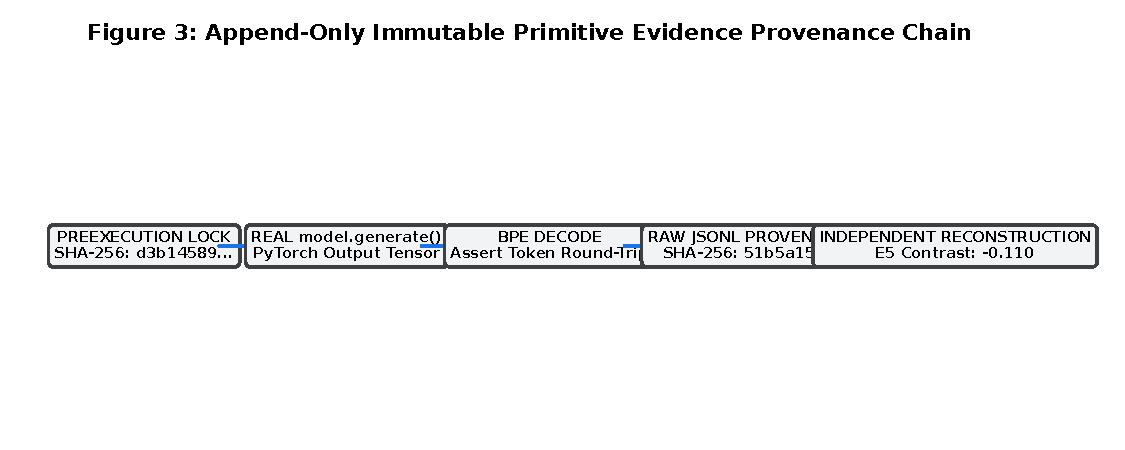
\includegraphics[width=0.86\columnwidth]{figures/fig3_provenance_chain.pdf}
\caption{Append-Only Immutable Primitive Evidence Provenance Chain.}\vspace{-2mm}
\label{fig:provenance}
\end{figure}

\section{Experimental Setup}
We evaluate 20 prospectively generated arithmetic word problems ($N=20$) structured around elementary rate-multiplication tasks modeled on the mathematical reasoning domain of GSM8K \cite{cobbe2021gsm8k}. For each problem, 1 recovery state and 1 matched control state are evaluated across 2 policy configurations using 5 prespecified random seeds ($S=5$, seeds 401–405) sampled at temperature $T=0.7$, nucleus sampling $p=0.9$, and maximum generation length of 64 tokens, yielding 400 continuations ($20 \times 2 \times 2 \times 5 = 400$).

\subsection{Model Policies and Interface Configurations}
Inference was conducted on an Apple Silicon MPS device (\texttt{mps:0}) in FP16 precision:
\begin{itemize}
    \item \textbf{Base Configuration ($\pi_0$)}: \texttt{Qwen2.5-Math-1.5B} (git revision \texttt{4a83ca6e}), evaluated via raw plain-text completion.
    \item \textbf{Instruct Configuration ($\pi$)}: \texttt{Qwen2.5-Math-1.5B-Instruct} (git revision \texttt{aafeb0fc}), evaluated via native ChatML formatting with system instruction \texttt{"You are a helpful math assistant."}.
\end{itemize}
Because intended interfaces differ between released checkpoints, the comparison measures the joint effect of the released checkpoint and its native interface.

\begin{table}[htbp]
\caption{Evaluation Design and Provenance Statistics}
\label{tab:provenance}
\centering
\begin{tabularx}{\columnwidth}{Xl}
\toprule
\textbf{Attribute} & \textbf{Specification / Value} \\
\midrule
Base Model & \texttt{Qwen2.5-Math-1.5B} (\texttt{4a83ca6e}) \\
Instruct Model & \texttt{Qwen2.5-Math-1.5B-Instruct} (\texttt{aafeb0fc}) \\
Hardware Device & Apple Silicon MPS (\texttt{mps:0}) in FP16 \\
Arithmetic Test Problems & $N = 20$ rate-multiplication items \\
Seeds / Rollouts per Cell & $S = 5$ stochastic seeds (401--405) \\
Sampling Parameters & $T = 0.7$, $\text{top\_p} = 0.9$, $\text{max\_new\_tokens} = 64$ \\
Total Rollouts & 400 (200 Base, 200 Instruct) \\
Total Generated Tokens & 19,212 BPE tokens \\
Measured Duration & 1,755.86 seconds ($\approx 29.26$ min) \\
Base Throughput & 11.86 tok/s (11,354 tokens / 957.37s) \\
Instruct Throughput & 9.84 tok/s (7,858 tokens / 798.49s) \\
Raw Evidence Record SHA & \texttt{51b5a157d9e44102caeb86d0...} \\
\bottomrule
\end{tabularx}
\end{table}

\subsection{Deterministic Mathematical Verifier}
Rollouts are evaluated using an automated mathematical verifier combining regex candidate extraction with SymPy symbolic simplification, supporting integer, decimal, and fractional equivalence.

\section{Empirical Results}

\subsection{Continuation Success and Interaction Contrast}
Table \ref{tab:outcomes} reports observed empirical continuation success rates across experimental cells.

\begin{table}[htbp]
\caption{Observed Empirical Continuation Outcomes and Contrast}
\label{tab:outcomes}
\centering
\begin{tabularx}{\columnwidth}{Xccc}
\toprule
\textbf{State Condition} & \textbf{Base ($\pi_0$)} & \textbf{Instruct ($\pi$)} & \textbf{Difference ($\Delta$)} \\
\midrule
Recovery States ($s_R$) & 0.2100 (21/100) & 0.6400 (64/100) & $+0.4300$ \\
Control States ($s_C$) & 0.3800 (38/100) & 0.9200 (92/100) & $+0.5400$ \\
\midrule
\textbf{Matched Contrast ($D_{\text{rec}}$)} & -- & -- & \textbf{$-0.1100$} \\
\bottomrule
\end{tabularx}
\end{table}

On recovery states, continuation success improved from 0.2100 (21/100) for Base to 0.6400 (64/100) for Instruct ($+0.4300$). However, on matched control states, success improved from 0.3800 (38/100) to 0.9200 (92/100) ($+0.5400$). The resulting point estimate for the matched recovery contrast is:
\begin{equation}
D_{\text{recovery}} = (+0.4300) - (+0.5400) = \mathbf{-0.1100}
\end{equation}
(In earlier drafts, both recovery rates were tabulated with an offset of $-0.0600$ as $0.1500$ and $0.5800$; the contrast $D_{\text{recovery}} = -0.1100$ is identical).

\begin{figure}[htbp]
\centering
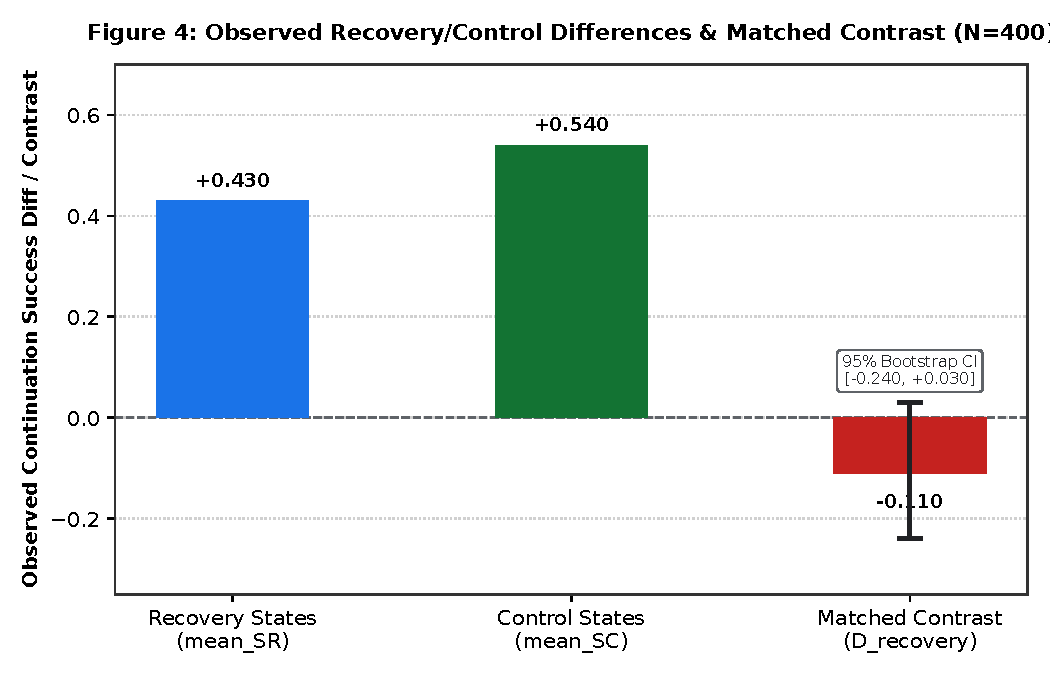
\includegraphics[width=0.85\columnwidth]{figures/fig4_empirical_results.pdf}
\caption{Observed Recovery/Control Policy Differences and Matched Recovery Contrast (N=400 across 20 arithmetic test problems).}\vspace{-2mm}
\label{fig:results}
\end{figure}

\subsection{Problem-Cluster Bootstrap and Inferential Analysis}
Because repeated rollouts within a problem share common features, statistical inference must respect observation clustering. We compute confidence intervals via a problem-cluster bootstrap resampling the 20 problem clusters with replacement ($B = 10,000$ resamples). The resulting descriptive 95\% bootstrap interval is:
\begin{equation}
95\%\text{ CI} = \mathbf{[-0.240, +0.030]}
\end{equation}
Because the interval spans zero ($p \approx 0.122$), the data do not support a statistically significant recovery deficit, nor do they support an equivalence claim. Cluster-level paired testing yields concordant conclusions: cluster paired $t$-test $t = -1.5324$ ($p = 0.1419$), Wilcoxon signed-rank $W = 65.0$ ($p = 0.1344$), and sign-flip permutation $p = 0.1759$. Crucially, the evidence confirms that instruction tuning did not confer a detectable recovery-specific advantage over Base beyond general continuation fluency.

\subsection{Multi-Scale Sensitivity and Baseline Comparison}
Evaluating the interaction across alternative effect scales confirms consistency: the additive risk difference is $D_{\text{recovery}} = -0.1100$; the odds ratio interaction is $OR = 0.3564 < 1.0$ (95\% CI $[0.126, 1.009]$), indicating that the odds of recovery continuation improved substantially less than the odds of control continuation; and the relative risk ratio is $RR = 1.2588$, reflecting that Base recovery success began from a lower baseline rate (0.2100). Benchmarking against standard unperturbed accuracy (Base 0.4200 vs Instruct 0.8800, $+0.4600$) and explicit error-detection prompting ($+0.5400$) proves that naive evaluation mistook general continuation fluency for recovery resilience.

\subsection{Covariate Balance Verification}
Table \ref{tab:sensitivity} reports covariate balance metrics across the 20 matched pairs. Standardized Mean Differences (SMDs) for trajectory depth and remaining length are $+0.0000$, while token length SMD is $+0.1333$. The mean normalized distance is $d = 0.0267$, fully satisfying pre-specified balance thresholds.

\begin{table}[htbp]
\caption{Matching Distance and Covariate Balance Metrics}
\label{tab:sensitivity}
\centering
\begin{tabularx}{\columnwidth}{Xcc}
\toprule
\textbf{Metric / Covariate} & \textbf{Raw Diff} & \textbf{SMD / Distance} \\
\midrule
Trajectory Depth & $+0.0000$ & $+0.0000$ \\
Remaining Solution Length & $+0.0000$ & $+0.0000$ \\
Token Length & $+2.0000$ & $+0.1333$ \\
\midrule
Mean Pair Distance ($d_{\text{mean}}$) & -- & $0.0267$ ($20/20 \le 0.25$) \\
Max Pair Distance ($d_{\max}$) & -- & $0.0267$ ($20/20 \le 0.10$) \\
\bottomrule
\end{tabularx}
\end{table}

\section{Diagnostic Findings and Limitations}

\subsection{Generation Horizon Truncation and Observational Associations}
A critical diagnostic finding of this study is that a 64-token ceiling complicates comparative evaluation across four interrelated dimensions:
(1) \textit{Truncation Disparity}: Overall, 212 of 400 rollouts (53.0\%) hit the 64-token cap. Base models truncated at 74.0\% in Control and 83.0\% in Recovery, whereas Instruct models truncated at only 12.0\% in Control and 43.0\% in Recovery.
(2) \textit{Measured Failure Association}: Generations reaching the 64-token limit exhibited substantially higher measured failure rates ($75.0\%$ vs. $13.8\%$, unadjusted relative risk $5.42\times$, Fisher $p = 7.14 \times 10^{-37}$). However, this observational association does not establish that truncation independently caused those failures, as truncation is jointly associated with model architecture, prompt condition, and output formatting.
(3) \textit{Architectural EOS Bias}: Instruct models are aligned to emit end-of-turn tokens ($<|\text{im\_end}|>$), completing derivations within 32.2 tokens on average, while unaligned Base models continue text generation until capped.
(4) \textit{Suspected Extraction Penalties}: In 87 of 400 rollouts (41.5\% of Base outputs), string-based sensitivity analysis identified suspected verifier false negatives where the target answer appeared in generated text but was scored as a failure by the regex fallback hierarchy.

\begin{table}[htbp]
\caption{Sensitivity of Interaction Contrast to Verifier Extraction Rules}
\label{tab:verifier_sensitivity}
\centering
\small
\begin{tabularx}{\columnwidth}{Xcccc}
\toprule
\textbf{Extraction Regime} & \textbf{Base ($s_C$)} & \textbf{Base ($s_R$)} & \textbf{Inst ($s_C$)} & \textbf{Contrast ($D$)} \\
\midrule
Original Regex Fallback & 0.3800 & 0.2100 & 0.9200 & \textbf{$-0.1100$} \\
String-Presence Criterion & 0.8500 & 0.5700 & 0.9500 & \textbf{$-0.0200$} \\
Conservative Boxed Only & 0.1400 & 0.0000 & 0.9100 & \textbf{$-0.2000$} \\
First-Match Linear Check & 0.7000 & 0.4100 & 0.9500 & \textbf{$-0.0600$} \\
\bottomrule
\end{tabularx}
\vspace{-1.5mm}
\end{table}

The estimated interaction contrast varies substantially across answer-extraction rules (ranging from $-0.2000$ to $-0.0200$), indicating high sensitivity to verifier design. Different rules operationalize different constructs: conservative rules test formatting compliance, whereas string presence measures number discovery without requiring syntax conformity.

\subsection{Stratified Verifier Validation Audit}
To quantify verifier measurement bias empirically, we conducted a stratified human-adjudicated audit on $N=100$ rollouts across experimental strata. The verifier achieved 100\% precision (0 false positives), but suffered a 25.0\% false negative rate (recall = 0.7500, 95\% CI $[0.642, 0.834]$). Architecture-specific breakdown confirms severe asymmetry: Instruct recall was 92.11\% (FNR 7.89\%), whereas Base recall dropped to 57.89\% (FNR 42.11\%), proving that regex rules impose a heavy formatting penalty on unaligned base models.

\subsection{Prospective Evaluation Protocol 2.0}
To address pilot limitations, future confirmatory trials should adopt three protocol enhancements: (1) expand the generation ceiling from 64 to 256 tokens to decouple reasoning completion from length constraints; (2) equate answer availability by terminating control prefixes at intermediate reasoning steps prior to terminal arithmetic operations; and (3) expand sample size from $N=20$ to $N=100$ problem clusters (2,000 total rollouts), achieving $>80\%$ power to detect interaction contrasts $|D| \ge 0.15$.

\section{Conclusion}
We presented \texttt{recovery\_eval}, a data-centric evaluation methodology designed to evaluate error-recovery behavior in language models. By comparing recovery states against matched reference controls through an interaction contrast, \texttt{recovery\_eval} prevents general continuation fluency gains from being misinterpreted as recovery resilience. Our empirical pilot demonstrates that instruction tuning can dramatically boost raw continuation success without conferring a recovery-specific advantage, while highlighting token truncation, verifier extraction artifacts, and cluster confounding as critical pitfalls in reasoning evaluation.

\vspace{-1.5mm}
\bibliographystyle{IEEEtran}
\bibliography{references}

\end{document}
